\documentclass{article}

\usepackage{amsmath}
\usepackage{amssymb}
\usepackage{bbm}
\usepackage[T1]{fontenc}
\usepackage{graphicx}
\usepackage{subfigure}
\usepackage{caption}
\usepackage{float}
\usepackage{geometry}
% \usepackage{nicematrix}
% \usepackage{minted}

\geometry{left = 3.18cm, top = 2.54cm, right = 3.18cm}

\title{\Large\bf MATH 629 Homework 1} 
\author{\normalsize Paul Zhang}
\date{\normalsize\today}

\begin{document}
\maketitle
\small
\section*{Problem 1}
The weights and biases are given by 
\begin{align*}
    \mathbf{W}^{(1)} & = \begin{bmatrix}
        -1 & 1 & 0 & 0 \\
        0 & -1 & 1 & 0 \\
        0 & 0 & -1 & 1 \\
    \end{bmatrix} \\
    \mathbf{b}^{(1)} & = \begin{bmatrix} 0 & 0 & 0\end{bmatrix} \\
    \mathbf{W}^{(2)} & = \begin{bmatrix} 1 & 1 & 1 \end{bmatrix} \\
    b^{(2)} & = -2.4
\end{align*}

\section*{Problem 2}
The dimensions of $X, Y, W, B$ are as follows (assuming that the number of features is $d$):
\begin{itemize}
    \item $X \in \mathbb{R}^{N \times d}$ 
    \item $Y = [y_1, y_2, \cdots, y_N]^T \in \mathbb{R}^{N\times 1}$
    \item $W \in \mathbb{R}^{d\times 1}$
    \item $B \in \mathbb{R}^{N\times 1}$
\end{itemize}
With the notations above, we can define $\mathcal{L}(Y ,T)$ as
$$ \mathcal{L}(Y, T) := [\mathcal{L}(y_1, t_1), \mathcal{L}(y_2, t_2), \cdots, \mathcal{L}(y_N, t_N)]^T 
\in \mathbb{R}^{N\times 1}$$
Accoringly, we have that
$$ \mathcal{E} = \frac{1}{N} \mathcal{L}(Y, T)^T \cdot e^{N\times 1} $$
and, obviously, 
$$ Y = XW + B $$
Therefore, the derivatives are computed as 
\begin{align*}
    \frac{\partial \mathcal{E}}{\partial Y} & = \frac{1}{N} \sin(Y - T) \\
    \frac{\partial \mathcal{E}}{\partial W} & = \frac{\partial \mathcal{E}}{\partial Y} \frac{\partial Y}
    {\partial W} = \frac{1}{N} X^T \sin(Y - T) \\
    \frac{\partial \mathcal{E}}{\partial B} & = \frac{\partial \mathcal{E}}{\partial Y} \frac{\partial Y}
    {\partial B} = \frac{1}{N} \sin(Y - T)
\end{align*}

\section*{Problem 3}
We start with showing that the absolute loss is indeed a squared loss with reassigned weights.
\begin{equation}
    \sum_{n = 1}^N \vert y_n - \mathbf{X_n}\beta \vert = \sum_{n = 1}^N \frac{1}{ \vert y_n - \mathbf{X_n}\beta \vert}
    (y_n - \mathbf{X_n}\beta)^2 =: \sum_{n = 1}^N s_n(y_n - \mathbf{X_n}\beta)^2
\end{equation}
In order to estimate the $s_n$'s, we can utilize the following algorithm:
\begin{itemize}
    \item Initialize OLS weights, $\beta^0$
    \item Compute residuals $\vert y_n - \mathbf{X_n}\beta \vert$
    \item Update weights $w^i_n$ with $w^i_n = \frac{1}{\vert y_n - \mathbf{X_n}\beta \vert}$
    \item Solve the WLS problem, $\beta^{i+1} = \mathrm{argmin}\sum_n w^i_n(y_n - X_n\beta^i)$
    \item Stop when $\vert \beta^{i+1} - \beta^i \vert < \epsilon$, where $\epsilon$ is a pre-determined threshold.
\end{itemize}

\section*{Problem 4}
\begin{figure}[H]
    \centering
    \caption{Implementation of XOR}
    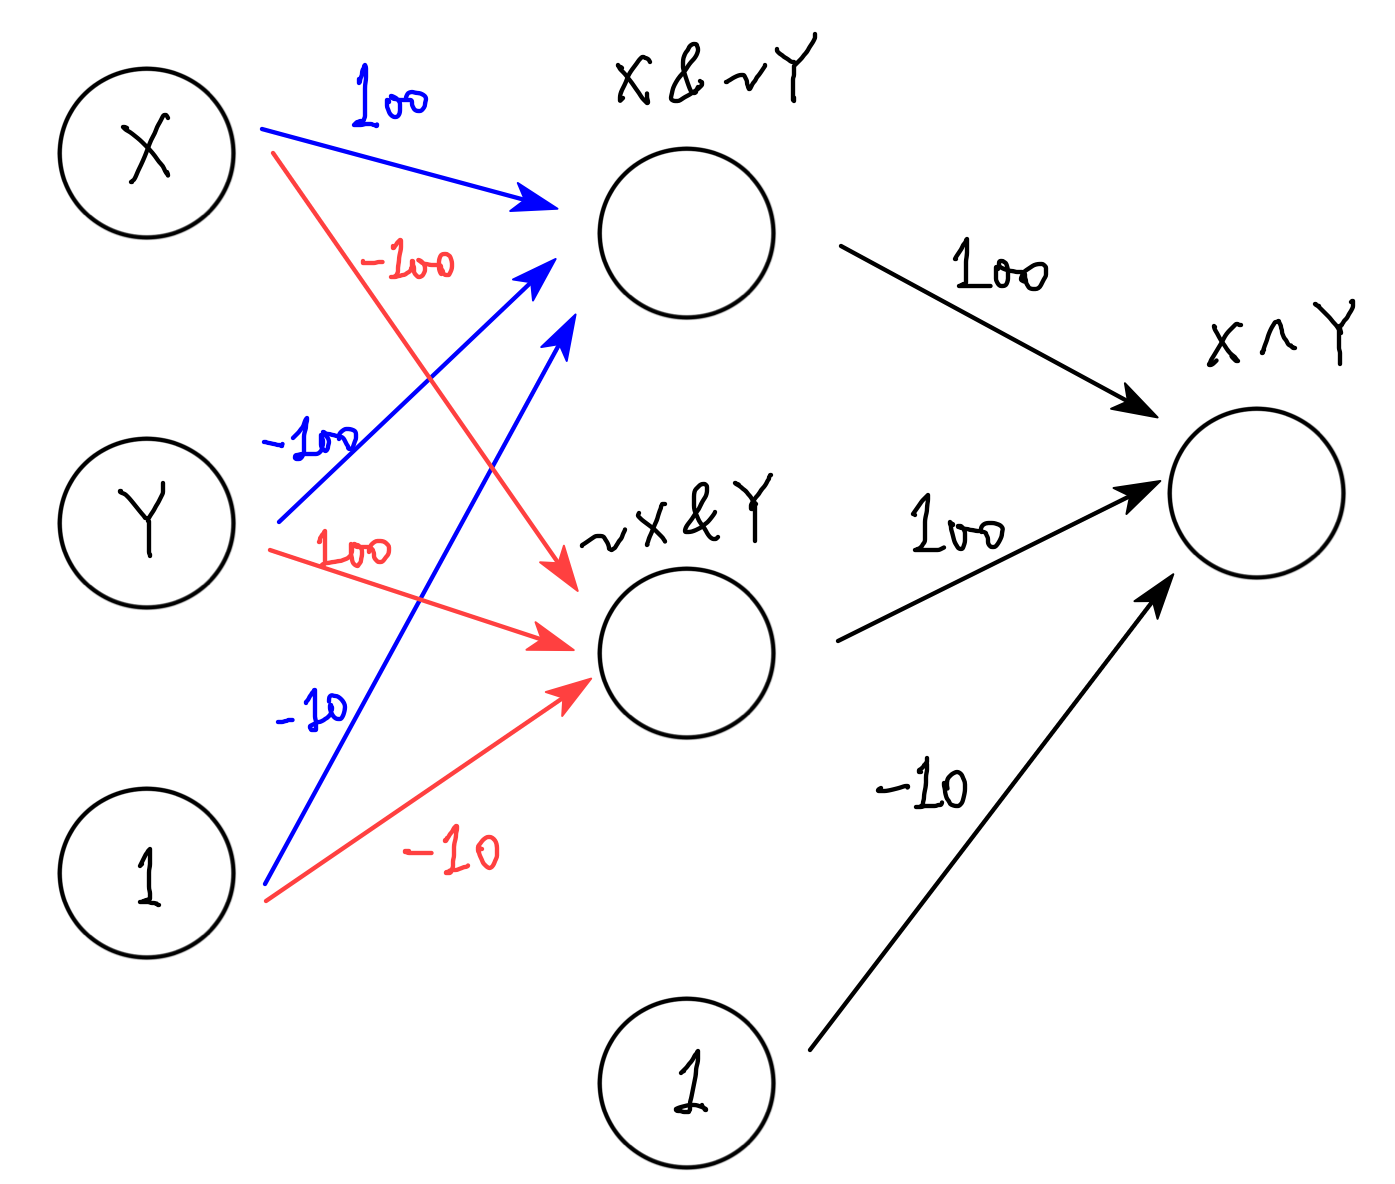
\includegraphics[width = .6\linewidth]{~/U-M/MATH629/machine_learning_for_finance_ii/hw1/pic/hw1_1.png}
\end{figure}

\end{document}